Given a value for $k$ and prediction point $x_{0}$ $KNN$ regression
firts identifies the $K$ training observations that are closed to 
$x_{0}$, represented by $\mathcal{N}_{0}$. It then estimates $f\left(
x_{0}\right)$ using the average of all the training responses in
$\mathcal{N}_{0}$.
\begin{center}
	\enc{$\widehat{f}\left(x_{0}\right)=\dfrac{1}{K}
	\su{{x_{i}\in\mathcal{N}_{0}}}{{}}y_{i}$}
\end{center}
\begin{figure}[H]
	\begin{center}
		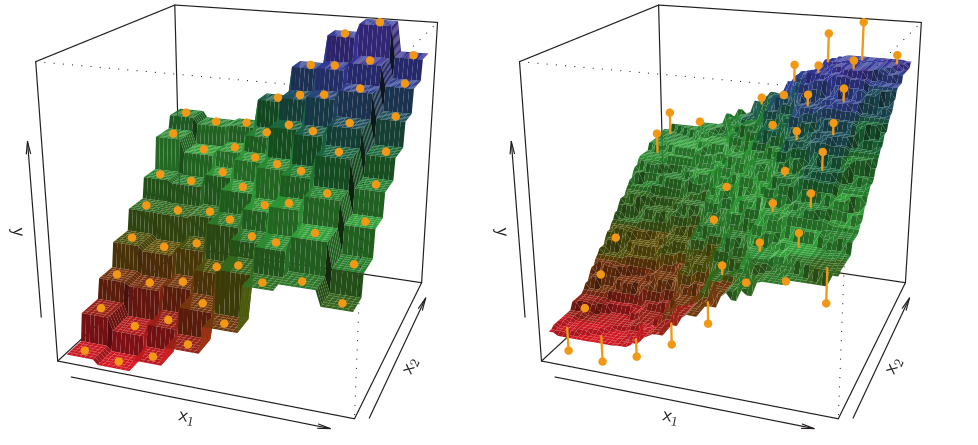
\includegraphics[width=\textwidth]{./chap/1chap/2sec/5images/1_KNNregression.png}
	\end{center}
	\caption{Plots of $\widehat{f}\left(X\right)$ using KNN 
	regression on a 2-dimensional data set with $64$ observations
	(orange dots). Left: $K=1$ results in a rough step function fit
	\\Right:$K=9$, averaging over $9$ observations results in a 
	much smaller region of constant prediction, and consequently
	a smoother fit.}
	\label{fig:fig 3.1}
\end{figure}
\begin{figure}[H]
	\begin{center}
		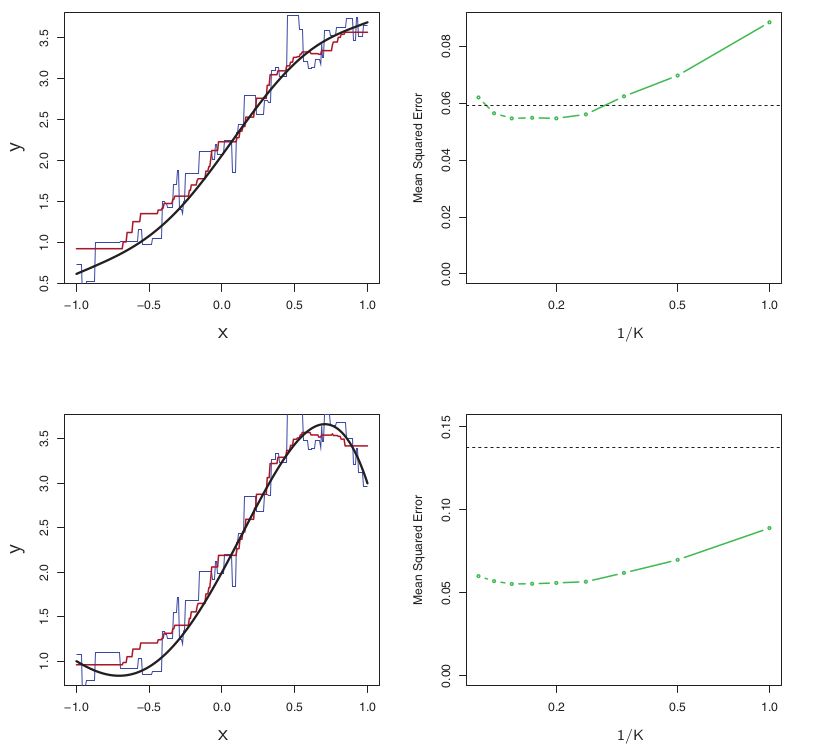
\includegraphics[width=\textwidth]{./chap/1chap/2sec/5images/2_comparisonKNNlinearRegression.png}
	\end{center}
	\caption{Top left: in a setting of slightly non-linear 
	relationship between $X$ and $Y$ (solid black line), the KNN
	fits with $K=1$ (blue) and $K=9$ (red) are displayed.\\ Top
	right: For the slightly non-linear data the test set MSE for
	least squares regression (horizontal black) and KNN with 
	various values of $\dfrac{1}{K}$ (green) are displayed.\\Bottom
	left and bottom right: as in the top of pannel, but with a
	strongly non-linear relationship between $X$ and $Y$.}
	\label{fig:fig 3.1}
\end{figure}
As a general rule, non-parametric method tend to outperform parametric
approaches when there is a small number of observation by prediction.
\begin{figure}[H]
	\begin{center}
		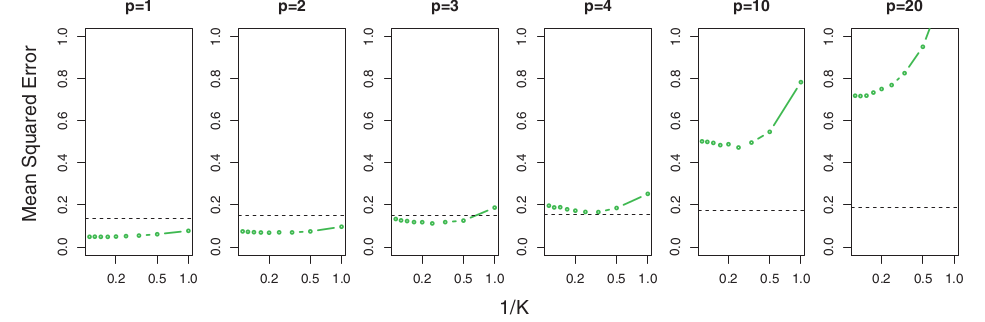
\includegraphics[width=\textwidth]{./chap/1chap/2sec/5images/3_TestMSE.png}
	\end{center}
	\caption{When $f$ is strongly non-linear.\\
	Test MSE for linear regression in black dashed lines,
	and these for KNN in green curves, as the number of prediction
	increases.}
	\label{fig:fig 3.1}
\end{figure}
